\section{Secagem de Refratários Monolíticos}\label{secagem}
De todas as etapas de processamento de materiais monolíticos com ligantes
hidráulicos, a secagem é uma das que mais toma tempo durante o processo de
reparo [REF LIVRO]. Devido a tal fator, há um grande potencial de ganho (em
termos de tempo de reparo e energia) na utilização de procedimentos de secagem
mais eficientes. Porém, qualquer dano provocado no material durante tal etapa
compromete a vida útil do refratário.

Além de tais desafios, garantir que a secagem, de fato, siga os procedimentos
recomendados pelo produtor (as curvas de secagem) é algo complexo dado
ineficiências do sistema de aquecimento (outro setor onde a simulação
computacional pode proporcionar grandes ganhos referentes a otimização do
sistema de aquecimento, bem como maior precisão e acurácia do sistema
controlador de temperaturas) e da falta de instrução dos operadores [REF LIVRO]. Soma-se o
fato de que muitas vezes as recomendações dadas pelo produtor são motivadas muito
mais pelo temor de ter que arcar com os custos de uma explosão ou de danos ao
equipamento devido problemas na secagem do que de fato fundamentos científicos e
testes experimentais.

Sendo assim há três estratégias comuns para a redução do risco de danos durante
o processo de secagem [REF LIVRO]:

\begin{enumerate}
\item Otimização da curva de secagem: \\ Para que a maior quantidade de água
  seja removida durante o regime de evaporação e não durante o regime de ebulição;
\item Alteração da microestrutura do material: \\ Para aumentar a permeabilidade e
  diminuir o nível de pressurização no interior do material;
\item Aumento da resistência mecânica: \\ Para que o material resista às tensões
  triaxiais decorrente da pressão do vapor de água.
\end{enumerate}

As próximas seções abordam cada uma dessas estratégias de forma mais
compreensiva, de forma a mostrar o estado da arte e como as simulações
computacionais poderiam complementar os estudos nesta área.

    \subsection{Curvas de secagem}
    Uma forma bastante comum no meio industrial para se definir uma curva de
    secagem é apresentado na Figura \ref{fig:industrial_HUC}.

\begin{figure}[ht]
\centering
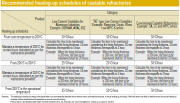
\includegraphics[width=\linewidth]{./figures/industrial_HUC.pdf}
\caption{Procedimento de secagem recomendado pela empresa AGC ceramics. Retirado de \cite{agc2016}. \label{fig:industrial_HUC}}
\end{figure}

    Observa-se que as taxas são definidas em diferentes intervalos de
    temperautra baseados aproximadamente nas temperautras de decomposição dos
    hidratos presentes no material. Além disso, o período de tempo em cada etapa
    é definido a partir da espessura do equipamento como uma maneira de se levar
    me consideração o efeito da distribuição de temperatura no interior do
    material.

    A crítica que se faz de tal procedimento é que tal correlação linear entre a
    temperatura e a espessura do componente não traduz os resultados
    experimentais e numéricos. Além disso, há a influência do próprio transporte
    de massa no interior do material nos perfis de temperatura o que pode gerar
    perfis completamente distintos.

    Tais orientações deveriam ser complementadas por resultados experimentais e
    simulações numéricas levando em conta não só as dimensões do refratário como
    também as condições de contorno, a geometria, a condutividade térmica e a
    permabilidade do material.

    Do ponto de vista empírico, ensaios de análise termogravimétrica podem ter
    grande importância para verificar se os intervalos de transofrmações
    propostos na curva de secagem, de fato correspondem com as trasnformações.

    \subsection{Aditivos para secagem}
     As recomendações 2 e 3 (alteração da microestrutura e aumento da
     resistência mecânica) podem ser implementadas através de aditivos
     adicionados na composição dos concretos. Dois casos específicos serão
     apresentados, são eles o uso de fibras poliméricas e fibras metálicas.
     Porém é importante salientar que inúmeras outras possibilidades também
     podem contribuir para o aumento de permeabilidade ou o aumento da
     resistência mecânica do material (como uso de diferentes sistemas ligantes,
     ou fases estabilizadas).

     As fibras metálicas apresentam a característica de ampliar a energia de
     fratura ao promover diferentes mecanismos de tenacificação como {\it
       crack-bridging}, {\it microcracking} e {\it pullout} [REF LIVRO]. Dessa
     maneira, há uma maior resistência ao dano por parte do material, de modo
     que as tensões devido a pressão do vapor não sejam capazes de promover o
     crescimento catastrófico das trincas. Além do efeito mecânico, o {\it
       microcracking} decorrente do {\it mismatch} dos coeficientes de expansão
     da matriz e das fibras metálicas, promove um aumento local da
     permeabilidade do material conforme reportado por Li et al \cite{li2019}.

     Por outro lado, as fibras poliméricas não apresentam quaisquer efeitos de
     tenacificação, inclusive promovendo defeitos de maiores dimenões o que
     diminui a resistêencia mecânica do material uma vez que tais polímeros são
     decompostos intencionalmente à baixas temperaturas (200$^\circ$C a
     300$^\circ$C) para promover o aumento da permeabiliade do material.

     Novamente, o uso da simulação computacional se faz importante uma vez que é
     necessário identificar a temperatura na qual a pressão no interior do
     material é máxima para selecionar o grade correto que apresente uma
     temperatura de composição coerente.

     Dessa forma justifica-se a busca por modelos númericos que possam garantir
     a otimização das curvas de secagem seja como um complemento às metodologias
     já sugeridas (como otimização da taxa de aquecimento, aumento da
     permebailidade ou aumento da resistência mecânica) ou ainda através de
     novas estratégias descobertas através da possibilidade de se obter os
     campos de pressão e temperatura no interior do material.
     
        
%%% Local Variables:
%%% mode: latex
%%% TeX-master: "TCC-Secagem"
%%% End:
